% This LaTeX was auto-generated from MATLAB code.
% To make changes, update the MATLAB code and export to LaTeX again.

\documentclass{article}

\usepackage[utf8]{inputenc}
\usepackage[T1]{fontenc}
\usepackage{lmodern}
\usepackage{graphicx}
\usepackage{color}
\usepackage{listings}
\usepackage{hyperref}
\usepackage{amsmath}
\usepackage{amsfonts}
\usepackage{epstopdf}
\usepackage{matlab}

\sloppy
\epstopdfsetup{outdir=./}
\graphicspath{ {./bsc_degree_fct_nova_grades_bar_plot_images/} }

\begin{document}

\begin{matlabcode}
courses = categorical({'Introduction to Programming (9 ECTS)', 'Linear Algebra and Analytic Geometry (6 ECTS)', 'Logic Systems (6 ECTS)', 'Mathematical Analysis I (6 ECTS)', 'Soft Skills for Science and Technology (3 ECTS)'});
grades = [16 13 12 12 16];
bar(courses, grades, 'FaceColor', [0.28 0.61 0.65], 'BarWidth', 0.5)
xlabel('Course')
ylabel('Grade [Scale of 0-20]')
ylim([0.0 20.0])
title('My BSc. Degree Grades (1st Year - 1st Semester @ FCT NOVA)'); 
\end{matlabcode}
\begin{center}
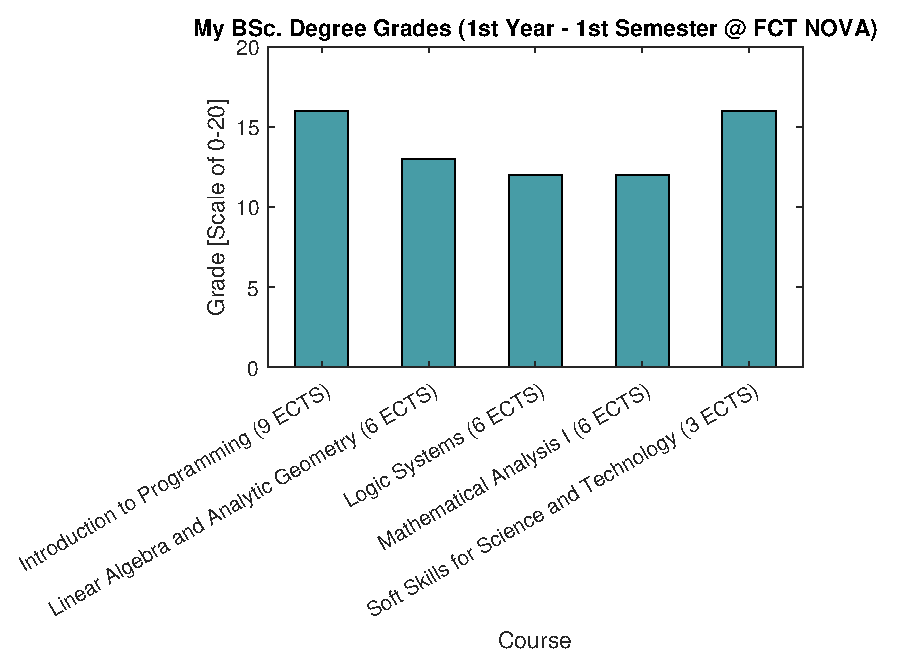
\includegraphics[width=\maxwidth{56.196688409433015em}]{figure_0}
\end{center}


\begin{matlabcode}
courses = categorical({'Computer Architecture (9 ECTS)', 'Discrete Mathematics (6 ECTS)', 'Mathematical Analysis II E (6 ECTS)', 'Object Oriented Programming (9 ECTS)'});
grades = [15 16 12 15];
bar(courses, grades, 'FaceColor', [0.12 0.73 0.52], 'BarWidth', 0.5)
xlabel('Course')
ylabel('Grade [Scale of 0-20]')
ylim([0.0 20.0])
title('My BSc. Degree Grades (1st Year - 2nd Semester @ FCT NOVA)'); 
\end{matlabcode}
\begin{center}
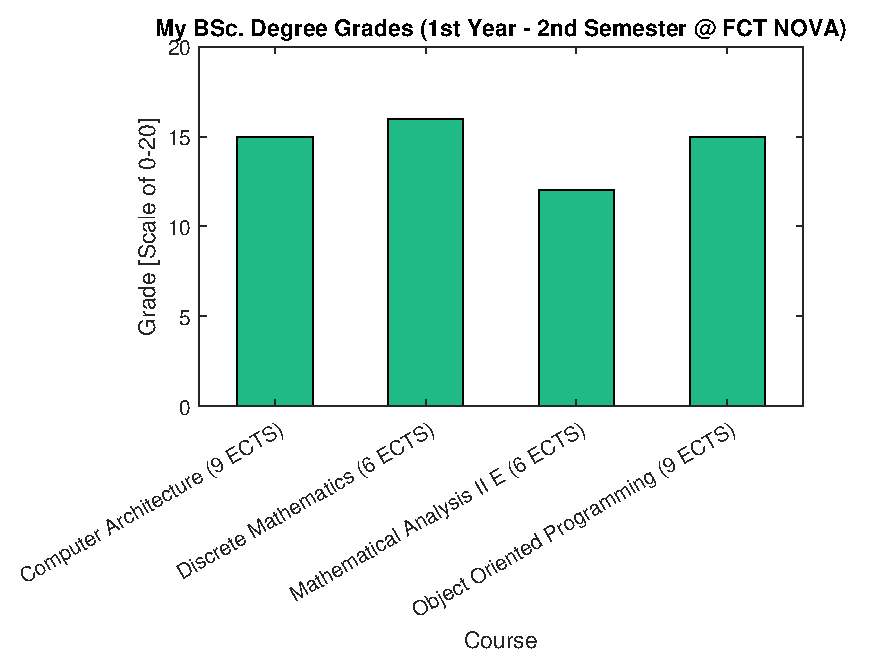
\includegraphics[width=\maxwidth{56.196688409433015em}]{figure_1}
\end{center}


\begin{matlabcode}
courses = categorical({'Algorithms and Data Structures (9 ECTS)', 'Computational Logic (6 ECTS)', 'Operating Systems Foundations (9 ECTS)', 'Physics (6 ECTS)'});
grades = [14 14 16 13];
bar(courses, grades, 'FaceColor', [0.12 0.73 0.52], 'BarWidth', 0.5)
xlabel('Course')
ylabel('Grade [Scale of 0-20]')
ylim([0.0 20.0])
title('My BSc. Degree Grades (2nd Year - 3rd Semester @ FCT NOVA)'); 
\end{matlabcode}
\begin{center}
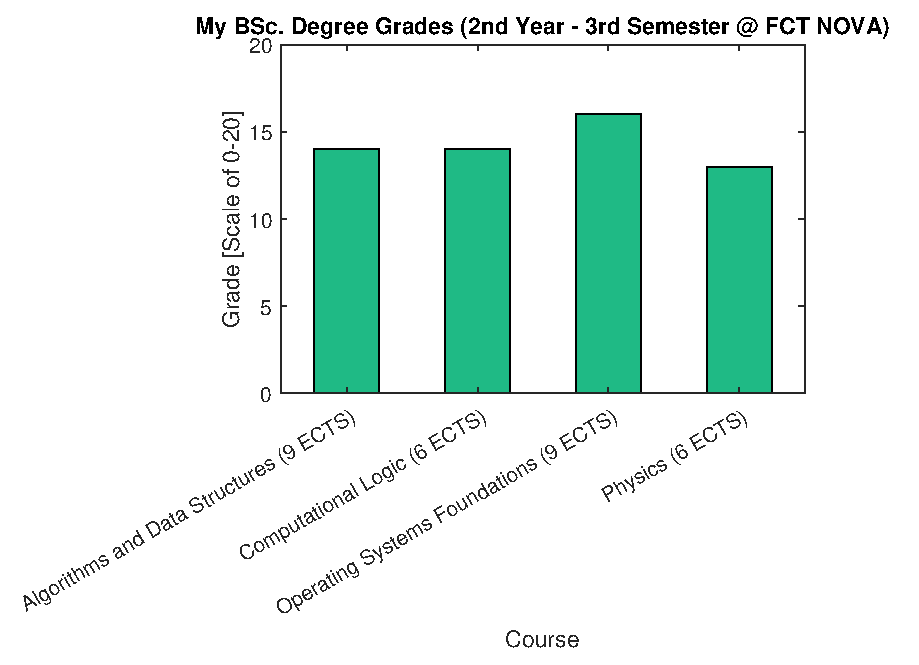
\includegraphics[width=\maxwidth{56.196688409433015em}]{figure_2}
\end{center}

\end{document}
